\documentclass[10pt]{article}

\usepackage[margin=1in]{geometry}
\usepackage{graphicx}
\usepackage{booktabs}
\usepackage{array}
\usepackage{tabularx}
\usepackage{microtype}
\usepackage{enumitem}
\usepackage{amsmath}
\usepackage[hidelinks]{hyperref}
\usepackage{caption}
\usepackage{subcaption}
\usepackage{xcolor}
\usepackage{tikz}
\usetikzlibrary{arrows.meta,positioning,shapes.geometric}

\setlength{\parindent}{0pt}
\setlength{\parskip}{3pt}
\setlist{nosep,leftmargin=*}
\captionsetup{font=small,skip=3pt}
\renewcommand{\arraystretch}{1.08}
\pagestyle{plain}

\title{\vspace{-1.4em}\textbf{DeEntropy: An AI Agent for Automated Dimension Reduction and Exploratory Data Analysis}\vspace{-0.6em}}
\author{Wenqing Zhu}
\date{}

\begin{document}
\maketitle
\vspace{-2.2em}

\section{Introduction and System Architecture}

Dimension reduction is central to exploratory analysis of high-dimensional
biomedical data, but an appropriate workflow depends strongly on the dataset.
Decisions such as whether to standardize features, preserve sparse
representations, introduce an intermediate linear reduction, or prioritize
local versus broader geometric structure are typically made manually. This
project develops \textbf{DeEntropy}, an automated agent that constructs,
executes, evaluates, and refines dimension-reduction workflows for previously
unseen datasets with minimal human intervention.

DeEntropy follows an iterative
\textit{Inspect $\rightarrow$ Plan $\rightarrow$ Preprocess $\rightarrow$
Execute $\rightarrow$ Evaluate $\rightarrow$ Reflect $\rightarrow$
Replan/Stop $\rightarrow$ Report} workflow. An \texttt{AnalysisDataset}
preserves the matrix, sample and feature identifiers, metadata, and optional
labels. The inspector produces a \texttt{DatasetProfile} containing dimensions,
feature types, missingness, sparsity, constant/near-constant features, scaling
characteristics, and count-like structure. The planner combines this profile
with a capability registry, feasibility information, computational budgets,
previous experiments, available artifacts, and reflection feedback to propose
a structured \texttt{AnalysisPlan}.

\begin{figure}[h!]
\centering
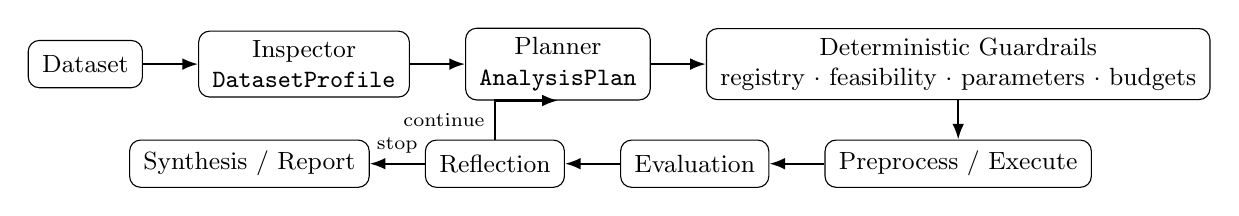
\begin{tikzpicture}[
  node distance=5mm and 7mm,
  box/.style={draw, rounded corners, align=center, minimum height=6mm,
              inner xsep=5pt, font=\small},
  guard/.style={draw, rounded corners, align=center, minimum height=9mm,
                inner xsep=5pt, font=\small},
  arr/.style={-{Latex[length=2mm]}, thick}
]
\node[box] (data) {Dataset};
\node[box, right=of data] (inspect) {Inspector\\\texttt{DatasetProfile}};
\node[box, right=of inspect] (plan) {Planner\\\texttt{AnalysisPlan}};
\node[guard, right=of plan] (guard)
    {Deterministic Guardrails\\registry $\cdot$ feasibility $\cdot$
    parameters $\cdot$ budgets};
\node[box, below=of guard] (exec) {Preprocess / Execute};
\node[box, left=of exec] (eval) {Evaluation};
\node[box, left=of eval] (reflect) {Reflection};
\node[box, left=of reflect] (report) {Synthesis / Report};

\draw[arr] (data) -- (inspect);
\draw[arr] (inspect) -- (plan);
\draw[arr] (plan) -- (guard);
\draw[arr] (guard) -- (exec);
\draw[arr] (exec) -- (eval);
\draw[arr] (eval) -- (reflect);
\draw[arr] (reflect) -- node[above,font=\scriptsize]{stop} (report);
\draw[arr] (reflect.north) |- node[pos=0.25,left,font=\scriptsize]{continue}
    (plan.south);
\end{tikzpicture}
\caption{DeEntropy architecture. The decision layer proposes analyses, while
deterministic code validates and executes them.}
\label{fig:architecture}
\end{figure}

Planning and numerical execution are deliberately separated. Deterministic
guardrails validate preprocessing compatibility and ordering, method
executability, hyperparameters, graph references and acyclicity,
representation compatibility, terminal-experiment budgets, and total
analysis-step limits. Only the executor performs numerical analysis.

DeEntropy supports two interchangeable decision providers: a deterministic
mock provider for reproducible, network-free execution and a structured OpenAI
provider for LLM-based planning and reflection. The finalized experiments
reported here use the deterministic provider so that analysis decisions are
reproducible. Regardless of provider, proposed plans conform to the same
Pydantic schemas and must pass the same deterministic validation before
execution.

\section{Agent Decision Making}

DeEntropy represents an analysis as a directed artifact graph rather than a
fixed list of algorithms. A workflow can therefore contain preprocessing,
reusable intermediate representations, and multiple terminal embeddings.
Intermediate steps do not count as independent terminal experiments and can be
reused across branches. This is particularly important for high-dimensional
or sparse data, where an expensive representation should not be recomputed for
every candidate embedding.

Method selection is profile-aware. The planner considers dimensionality,
storage representation, sparsity, scaling, count-like structure,
computational feasibility, and registered method strengths and limitations.
Hyperparameters are constrained by method-specific rules and dataset
dimensions. The system therefore chooses among suitable methods instead of
applying every available algorithm indiscriminately.

Terminal embeddings are evaluated using trustworthiness,
$k$-nearest-neighbor (kNN) preservation, and Pearson and Spearman correlations
of pairwise distances. The implementation uses scikit-learn for the core
PCA/manifold-learning methods and trustworthiness calculation
\cite{pedregosa2011,sklearn_manifold}, with UMAP provided by the implementation
based on McInnes et al. \cite{mcinnes2018}.

When labels are available, silhouette score and neighborhood label agreement
are computed only as post-hoc external validation; labels are excluded
from preprocessing, method selection, hyperparameter selection, and embedding
fitting. The reflector uses completed experiments and their metrics to decide
whether another strategy is warranted. Final synthesis does not average
heterogeneous metrics into a single score. Instead, it separately recommends
embeddings for local-neighborhood exploration, broader pairwise structure, and,
when available, post-hoc label alignment.

\section{Experimental Results}

The same DeEntropy architecture was evaluated on two real gene-expression
datasets with substantially different representations: the UCI Gene Expression
Cancer RNA-Seq dataset, derived from the TCGA PANCAN collection
\cite{uci_tcga}, and the PBMC3K count matrix distributed for the Scanpy PBMC3K
tutorial \cite{zenodo_pbmc,tenx_pbmc}. Table~\ref{tab:workflows} summarizes the
autonomous workflows.

\begin{table}[h!]
\centering
\caption{Final workflows selected by DeEntropy.}
\label{tab:workflows}
\small
\begin{tabularx}{\textwidth}{>{\bfseries}p{0.20\textwidth}XX}
\toprule
 & Dataset 1: Cancer RNA-seq & Dataset 2: PBMC3K \\
\midrule
Samples $\times$ features
    & $801\times20{,}531$
    & $2{,}700\times32{,}738$ \\
Storage / labels
    & Dense / 5 classes
    & Sparse CSR / none \\
Key characteristic
    & $p/n=25.63$
    & 97.4\% sparse, count-like \\
Preprocessing
    & Constants $\rightarrow$ variance selection $\rightarrow$ standardization
    & Constants $\rightarrow$ total normalization $\rightarrow$ log1p
      $\rightarrow$ variance selection \\
Reusable intermediate
    & PCA, 29 components
    & Truncated SVD, 52 components \\
Terminal methods
    & Isomap; Spectral Embedding
    & UMAP; PCA \\
Local recommendation
    & Spectral Embedding
    & UMAP \\
Broader structure
    & Isomap
    & PCA \\
\bottomrule
\end{tabularx}
\end{table}

\subsection{Dataset 1: Gene Expression Cancer RNA-seq}

Dataset 1 contained 801 samples and 20,531 numeric features, including 267
constant and 210 near-constant features. DeEntropy removed the constant
features, retained the top 4,056 variance-ranked features, and standardized
them. It then constructed a reusable PCA representation with 29 components
\cite{jolliffe2016} and evaluated Isomap \cite{tenenbaum2000} and Spectral
Embedding (Laplacian Eigenmaps) \cite{belkin2003} as terminal methods.

Relative to the PCA-29 parent representation, Spectral Embedding better
preserved local structure: trustworthiness was \textbf{0.957} and kNN
preservation was \textbf{0.299}, compared with 0.942 and 0.242 for Isomap.
In the separate post-hoc label-based evaluation, Spectral Embedding also showed
stronger class alignment (silhouette \textbf{0.883}; neighborhood label
agreement \textbf{0.995}) than Isomap (0.758; 0.989). Isomap better preserved
broader pairwise geometry relative to the same parent representation, with
Pearson/Spearman distance correlations of \textbf{0.753/0.754}, versus
0.680/0.724 for Spectral Embedding. DeEntropy therefore recommended Spectral
Embedding for local exploration and post-hoc label alignment, and Isomap as
the broader pairwise-structure reference.

\begin{figure}[h!]
\centering
\begin{subfigure}[t]{0.49\textwidth}
\centering
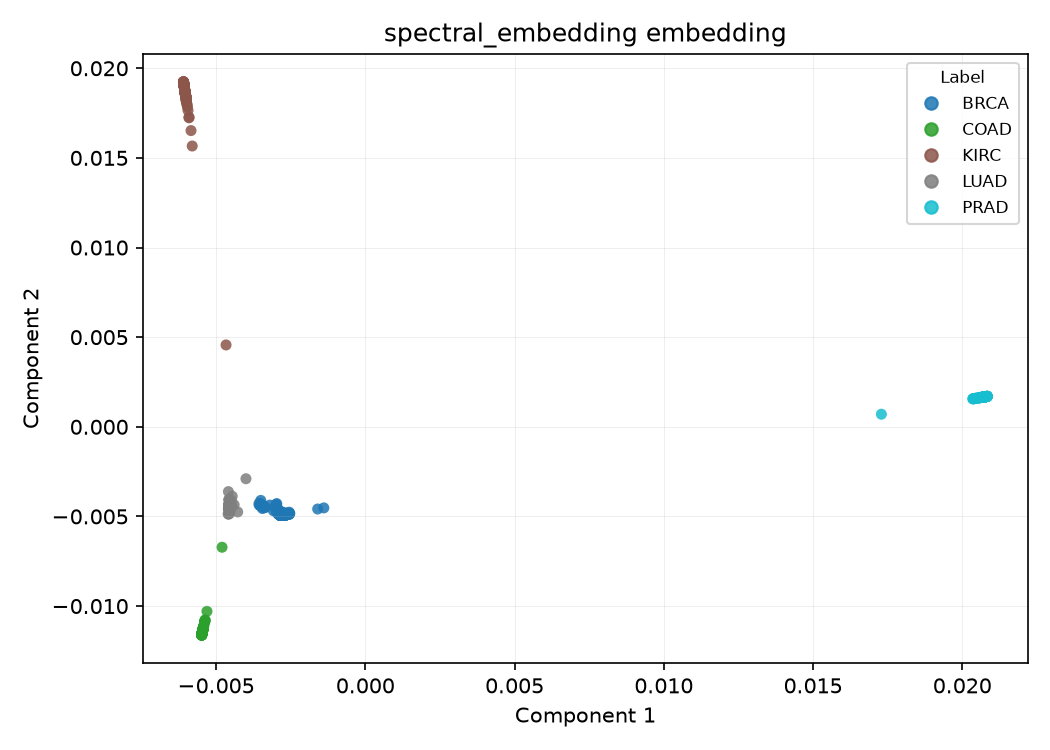
\includegraphics[width=\linewidth]
    {outputs/dataset_1/plots/spectral_embedding_embedding.png}
\caption{Spectral Embedding: preferred for local structure and post-hoc class
alignment.}
\end{subfigure}\hfill
\begin{subfigure}[t]{0.49\textwidth}
\centering
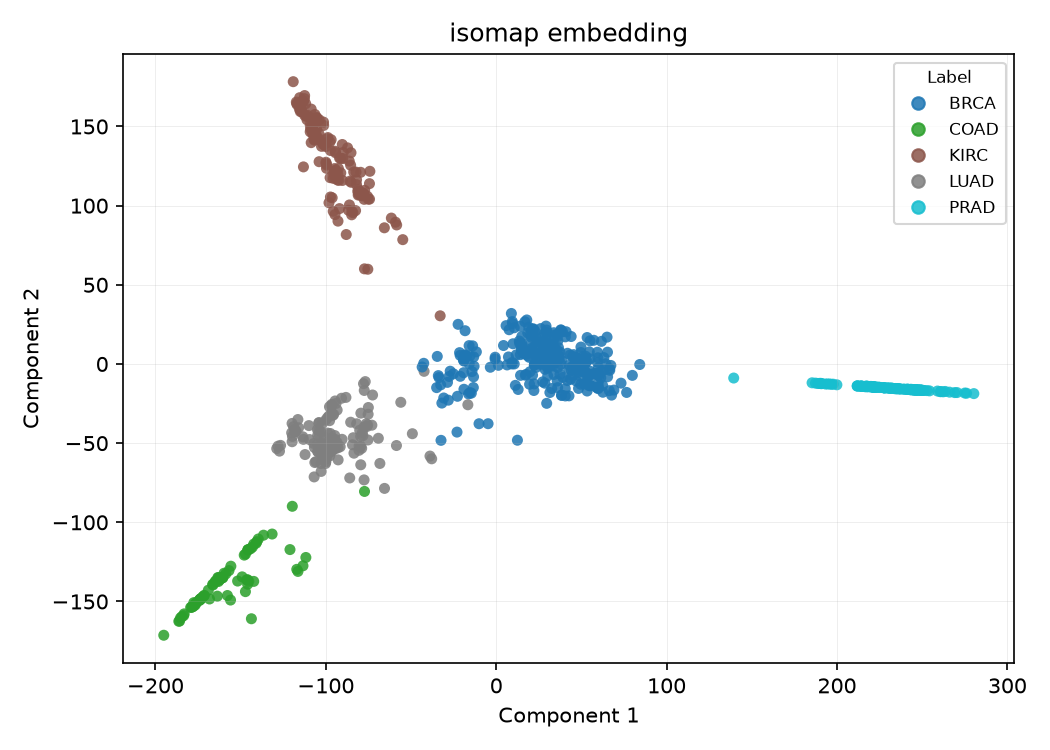
\includegraphics[width=\linewidth]
    {outputs/dataset_1/plots/isomap_embedding.png}
\caption{Isomap: preferred as the broader pairwise-structure reference.}
\end{subfigure}
\caption{Dataset 1 terminal embeddings. Class labels are used for visualization
and post-hoc evaluation only.}
\label{fig:dataset1}
\end{figure}

\subsection{Dataset 2: PBMC3K}

Dataset 2 contained 2,700 samples and 32,738 features in a 97.4\% sparse,
nonnegative count matrix. DeEntropy preserved sparse storage, removed 16,104
constant features, applied generic sample-total normalization, followed by
sparse-safe \texttt{log1p}, and retained 9,402 variance-ranked features. The
sparse root was never fully densified. The agent selected noncentered Truncated
SVD with 52 components as a reusable intermediate, using a randomized low-rank
decomposition \cite{halko2011}, followed by UMAP \cite{mcinnes2018} and PCA
\cite{jolliffe2016} terminal experiments.

Relative to the shared SVD-52 parent representation, UMAP provided better local
preservation, with trustworthiness \textbf{0.922} and kNN preservation
\textbf{0.213}, versus 0.865 and 0.088 for PCA. PCA better preserved broader
pairwise relationships, with Pearson/Spearman distance correlations of
\textbf{0.908/0.890}, versus 0.735/0.786 for UMAP. DeEntropy therefore
recommended UMAP for local-neighborhood exploration and PCA as the broader
pairwise-structure reference. External validation was unavailable because no
class or cell-type labels were provided. Root-fidelity metrics were
intentionally omitted because the current evaluator would require densifying
the sparse root.

\begin{figure}[h!]
\centering
\begin{subfigure}[t]{0.49\textwidth}
\centering
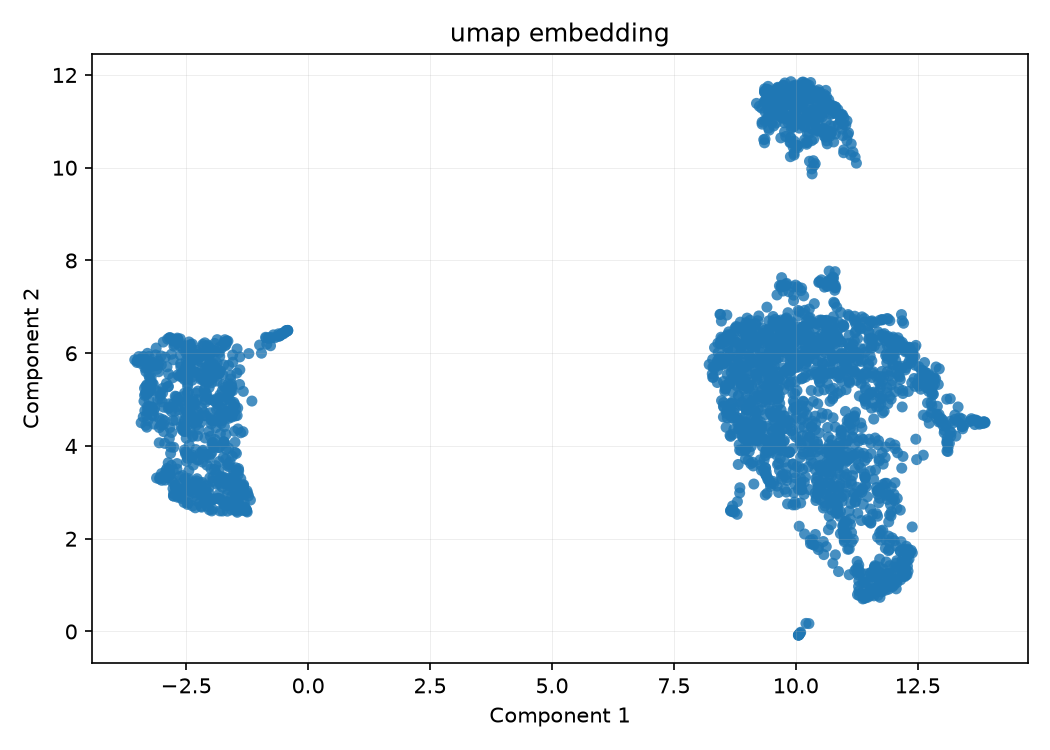
\includegraphics[width=\linewidth]
    {outputs/dataset_2/plots/umap_embedding.png}
\caption{UMAP: preferred for local-neighborhood exploration.}
\end{subfigure}\hfill
\begin{subfigure}[t]{0.49\textwidth}
\centering
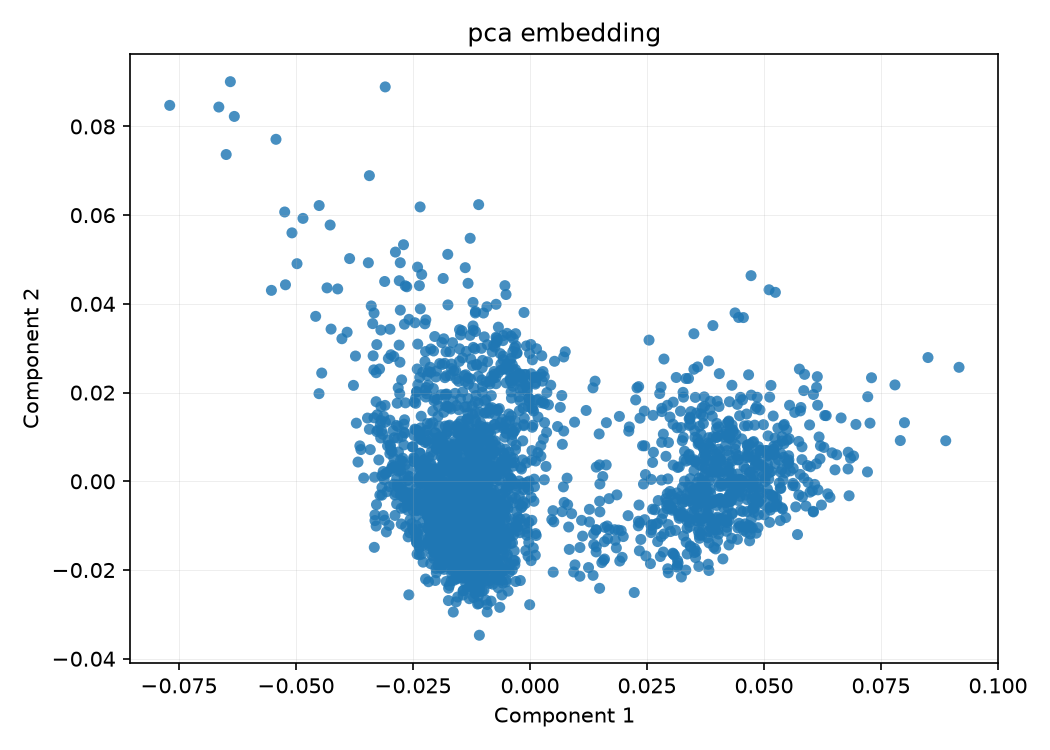
\includegraphics[width=\linewidth]
    {outputs/dataset_2/plots/pca_embedding.png}
\caption{PCA: preferred as the broader pairwise-structure reference.}
\end{subfigure}
\caption{Dataset 2 terminal embeddings after the shared Truncated SVD
representation.}
\label{fig:dataset2}
\end{figure}

Across both datasets, the results illustrate a central design choice:
DeEntropy does not force a single ``best'' embedding. Local-neighborhood
preservation and broader pairwise-structure preservation can favor different
methods, so recommendations are tied to the intended exploratory purpose.

\section{Strengths and Limitations}

A principal strength of DeEntropy is the separation of adaptive
decision making from deterministic statistical execution. Dataset
characteristics influence preprocessing and method selection, while explicit
capability definitions and validation prevent unsupported methods, incompatible
representations, invalid hyperparameters, and excessive computational plans
from being executed. The artifact graph enables exact intermediate reuse with
provenance, and the same architecture successfully handled both a dense labeled
dataset and a sparse unlabeled count matrix. Sample identifiers,
configurations, analysis histories, metrics, and random seed 42 are retained
to support reproducibility.

Important limitations remain. Deterministic mock planning relies on heuristic
rules, while real LLM proposals may be uncertain or invalid and therefore
require deterministic rejection. The two-terminal-experiment budget allows
adaptive comparison but not exhaustive method or hyperparameter search.
Diffusion Maps and GPLVM are registered but not executable. Preprocessing is
intentionally general rather than domain-specialized: DeEntropy does not
perform specialized highly variable gene modeling, clustering, or biological
annotation. Sparse-root fidelity is unavailable when evaluation would require
full densification, and Dataset 2 lacks labels for external validation.
Finally, the reported metrics measure structural preservation and should not
be interpreted as biological truth or causality.

\section{Toward a General Biomedical Data Analysis Agent}

Project 1 is the first stage of a four-project sequence covering
(1) dimension reduction and exploratory analysis,
(2) generative modeling,
(3) multimodality learning, and
(4) general AI-agent-based analysis of complex biomedical data.
DeEntropy was therefore designed around reusable components---dataset
representation, inspection, planning, deterministic validation, execution,
evaluation, reflection, and artifact provenance---rather than as an isolated
dimension-reduction pipeline.

Future projects will extend the registered analytical capabilities while
preserving this control architecture. The next stage will introduce generative
modeling tools, followed by multimodal analysis and ultimately coordination of
multiple analytical modules within a general biomedical data-analysis agent.
A further methodological direction is to incorporate Bayesian reasoning into
the decision layer: uncertainty about competing analysis strategies
could be represented explicitly and updated using results from completed
experiments. Bayesian or LLM-based reasoning would propose and prioritize
actions, while deterministic guardrails would remain responsible for
validating and executing them.

\section{Conclusion}

DeEntropy demonstrates that dimension-reduction analysis can be formulated as
an iterative agentic decision process rather than a fixed benchmarking
pipeline. Across two substantially different biomedical datasets, it
autonomously constructed feasible workflows, adapted preprocessing and method
selection to the data representation, evaluated competing embeddings, reused
intermediate computations, and produced purpose-specific recommendations.
The resulting architecture provides a reusable foundation for extending the
agent beyond dimension reduction in subsequent projects.

\clearpage

\small
\begin{thebibliography}{99}

\bibitem{uci_tcga}
UCI Machine Learning Repository.
\newblock \emph{Gene Expression Cancer RNA-Seq}.
\newblock Donated 2016. Gene-expression dataset containing 801 samples and
20,531 expression features across BRCA, KIRC, COAD, LUAD, and PRAD.
\newblock
\url{https://archive.ics.uci.edu/dataset/401/gene+expression+cancer+rna+seq}.

\bibitem{zenodo_pbmc}
Theis Lab / Scanpy tutorial data.
\newblock \emph{Training data for ``Clustering 3K PBMCs with Scanpy''}.
\newblock Zenodo, 2019. DOI:
\href{https://doi.org/10.5281/zenodo.3581213}{10.5281/zenodo.3581213}.
\newblock Files used in this project:
\texttt{matrix.mtx}, \texttt{barcodes.tsv}, and \texttt{genes.tsv}.

\bibitem{tenx_pbmc}
10x Genomics.
\newblock \emph{3k PBMCs from a Healthy Donor}.
\newblock Chromium/GemCode single-cell gene-expression dataset, originally
released in 2016.
\newblock
\url{https://www.10xgenomics.com/datasets/3-k-pbm-cs-from-a-healthy-donor-1-standard-1-0-0}.

\bibitem{jolliffe2016}
I. T. Jolliffe and J. Cadima.
\newblock Principal component analysis: a review and recent developments.
\newblock \emph{Philosophical Transactions of the Royal Society A},
374(2065):20150202, 2016.
\newblock doi:10.1098/rsta.2015.0202.

\bibitem{tenenbaum2000}
J. B. Tenenbaum, V. de Silva, and J. C. Langford.
\newblock A global geometric framework for nonlinear dimensionality reduction.
\newblock \emph{Science}, 290(5500):2319--2323, 2000.
\newblock doi:10.1126/science.290.5500.2319.

\bibitem{belkin2003}
M. Belkin and P. Niyogi.
\newblock Laplacian Eigenmaps for dimensionality reduction and data
representation.
\newblock \emph{Neural Computation}, 15(6):1373--1396, 2003.
\newblock doi:10.1162/089976603321780317.

\bibitem{halko2011}
N. Halko, P. G. Martinsson, and J. A. Tropp.
\newblock Finding structure with randomness: probabilistic algorithms for
constructing approximate matrix decompositions.
\newblock \emph{SIAM Review}, 53(2):217--288, 2011.
\newblock doi:10.1137/090771806.

\bibitem{mcinnes2018}
L. McInnes, J. Healy, and J. Melville.
\newblock UMAP: Uniform Manifold Approximation and Projection for Dimension
Reduction.
\newblock arXiv:1802.03426, 2018.
\newblock \url{https://arxiv.org/abs/1802.03426}.

\bibitem{pedregosa2011}
F. Pedregosa et al.
\newblock Scikit-learn: Machine Learning in Python.
\newblock \emph{Journal of Machine Learning Research},
12:2825--2830, 2011.

\bibitem{sklearn_manifold}
Scikit-learn developers.
\newblock \emph{Manifold learning API documentation}.
\newblock Documentation for Isomap, Spectral Embedding, MDS, LLE, t-SNE, and
trustworthiness.
\newblock \url{https://scikit-learn.org/stable/api/sklearn.manifold.html}.

\end{thebibliography}

\end{document}